\documentclass[a4paper, 12pt, titlepage]{article}

\usepackage[utf8]{inputenc}
\usepackage{geometry}
\usepackage{polski}
\usepackage{graphicx} 
\usepackage{float} 
\usepackage{etoolbox,refcount}
\usepackage{multicol}
\usepackage{fancyhdr}
\usepackage{listings}
\usepackage{amsmath}
\usepackage{tabularx}

\pdfsuppresswarningpagegroup=1
\newgeometry{left=2.5cm, right=2.5cm, bottom=2.5cm, top=2.5cm}

\lstset{
    language=Matlab,
    basicstyle=\ttfamily,
    keepspaces=true,
    frame=single,
    tabsize=4,
    showspaces=false,
    showstringspaces=false,
    extendedchars=true,
    inputencoding=utf8,
    literate={ó}{{\'o}}1 {ę}{{\k{e}}}1 {ł}{{\l{}}}1 {ż}{{\.z}}1
        {ś}{{\'s}}1 {ć}{{\'c}}1 {ą}{{\k{a}}}1 {ź}{{\'z}}1 {ń}{{\'n}}1
}
\author{Adrian Jałoszewski}
\title{Ćwiczenie 6: Rozpoznawanie obrazów w środowisku MATLAB}
\date{13 listopada 2017}

\begin{document}
    \maketitle
    \section{SURF} 
        SURF -- speeded up robust features -- zainspirowany SIFT.  Cechy:
        \begin{itemize}
            \item[--] szybki (kilkakrotnie szybszy od SIFT)
            \item[--] odporniejszy od SIFT na transformacje obrazu
            \item[--] opis cech na podstawie sumy falek Haara w okolicy
                punktów zainteresowania
            \item[--] wykorzystuje obraz całgowany (integral image) dla
                optymalizacji
            \item[--] przez zastosowanie piramidowania odporny na skalowanie
            \item[--] aproksymuje rozmycie Gaussa -- przyśpieszenie w stosunku
                do SIFT
            \item[--] wykorzystuje macierz Hessego do znalezienia punktów 
                zainteresowania
            \item[--] nieodporny na rozmycia obrazu
        \end{itemize}
    \section{Wyznaczenie cech charakterystycznych dla wzorców}
        \subsection{Nazwy plików}
\begin{lstlisting}
file_names = { 
    'magneB6_wzorzec.jpg'
    'NoSpa_wzorzec.jpg'
    'chlorchinaldin_wzorzec.jpg'
    'vitaminumB_wzorzec.jpg'
};
\end{lstlisting}
        \subsection{Wykrywanie cech SURF}
\begin{lstlisting}
modelData = struct('objImage', [], ...
                'objValidPoints', [], ...
                'objFeatures', []);

for i=1:length(file_names)
    file_name = file_names{i};
    image = rgb2gray(imread(file_name));
    surfFeatures = detectSURFFeatures(image);
    strongest = surfFeatures.selectStrongest(100);
    [features, validPoints] = ... 
        extractFeatures(image, strongest);

    modelData(i).objImage = image;
    modelData(i).objValidPoints = validPoints;
    modelData(i).objFeatures = features;
end

save modelData
\end{lstlisting}
        W ten sposób zostały wykryte następujące 100 najsilniejszych cech:
        \begin{figure}[H]
            \centering
            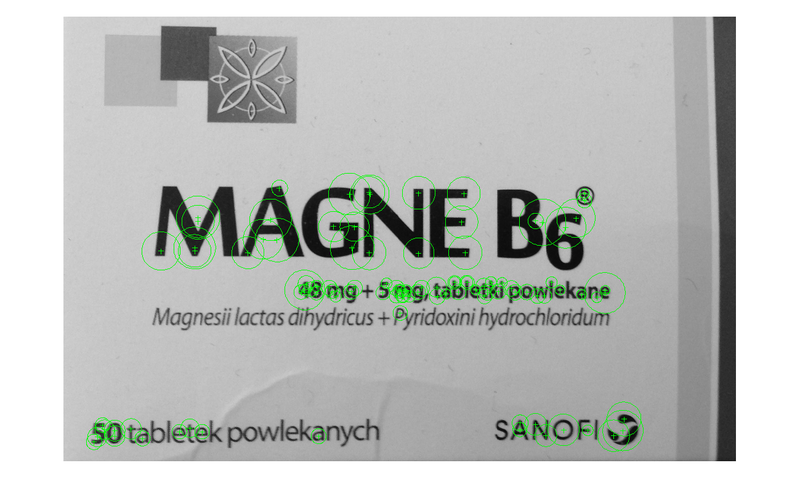
\includegraphics[width=\linewidth]{first/a.png}
        \end{figure}
        \begin{figure}[H]
            \centering
            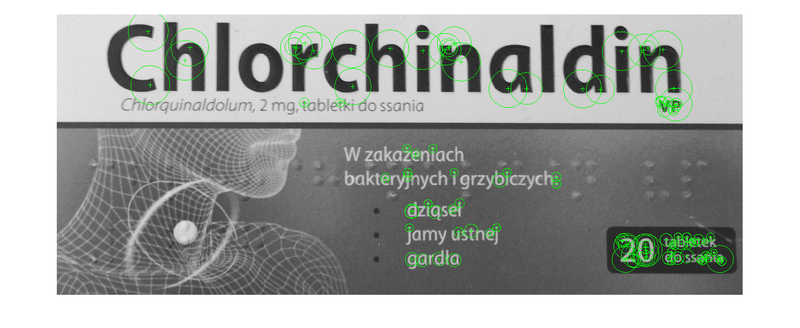
\includegraphics[width=\linewidth]{first/chlorchinaldin.png}
        \end{figure}
        \begin{figure}[H]
            \centering
            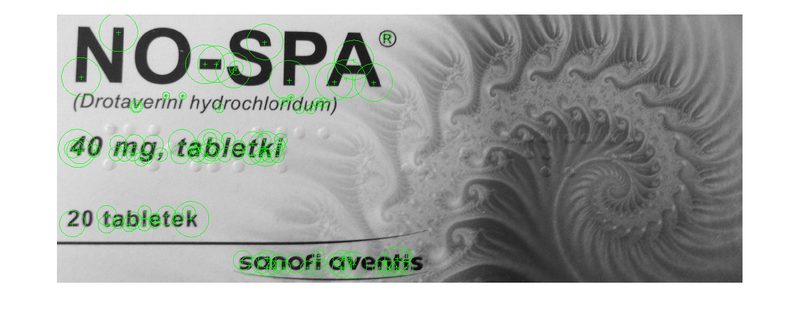
\includegraphics[width=\linewidth]{first/nospa.png}
        \end{figure}
        \begin{figure}[H]
            \centering
            
\includegraphics[width=\linewidth]{first/vitaminum.png}
        \end{figure}
    \section{Klasyfikacja obiektów}
        \subsection{Wczytywanie obiektu}
\begin{lstlisting}
load modelData
objImage = modelData(wzorzecNr).objImage;
objValidPoints = modelData(wzorzecNr).objValidPoints;
objFeatures = modelData(wzorzecNr).objFeatures;
\end{lstlisting}
        \subsection{Wczytywanie obrazu}
\begin{lstlisting}
nazwa1 = [baseFileName, num2str(i), fileExtension];

disp(nazwa1);
RGB=imread(nazwa1);
sceneImage = rgb2gray(RGB); 
\end{lstlisting}
        \subsection{Wykrywanie cech SURF i dobieranie parami ze wzorcem}
\begin{lstlisting}
surfFeatures = detectSURFFeatures(sceneImage);
strongest = selectStrongest(surfFeatures, 100);
[sceneFeatures, sceneValidPoints] = ...
    extractFeatures(sceneImage, strongest);

featurePairs = matchFeatures(objFeatures, sceneFeatures, ...
                             'unique',true);
matchedObjPoints = objValidPoints(featurePairs(:, 1), :);
matchedScenePoints = sceneValidPoints(featurePairs(:, 2), :);
\end{lstlisting}
        \subsection{Wizualizacja}
\begin{lstlisting}
if visON==1
    figure;
    showMatchedFeatures(objImage, sceneImage, ...
    matchedObjPoints, matchedScenePoints, 'montage');
    print(['second/', num2str(wzorzecNr), ...
        '_',num2str(i) , '_obraz'], '-dpng')
end
\end{lstlisting}
            \begin{figure}[H]
                \centering
                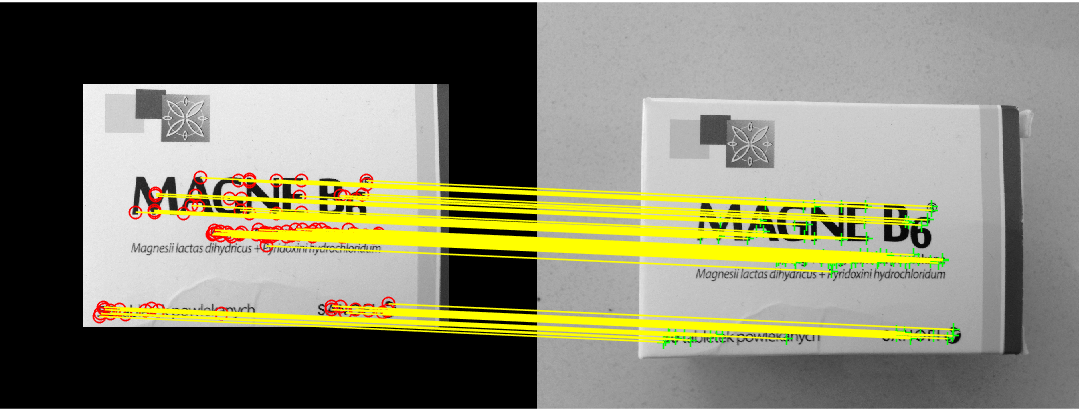
\includegraphics[width=\linewidth]{second/1_1_obraz.png}
            \end{figure}
            \begin{figure}[H]
                \centering
                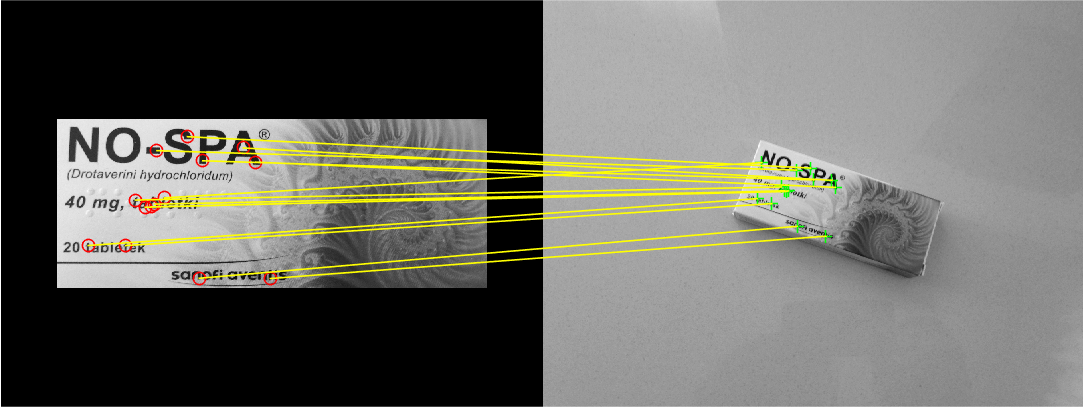
\includegraphics[width=\linewidth]{second/2_7_obraz.png}
            \end{figure}
            Algorytm zwraca szczególnie uwagę na krawędzie liter i probuje
            je dopasować pomiędzy obrazami. W przypadku jak te krawędzie są
            rozmazane, mimo tego, że ma doczynienia z tymi samymi 
            przedmiotami nie jest w stanie ich rozróżnić. Obrazy, które
            zawierają te same opakowania zawierają wiele wspólnych wykrytych
            cech, obrazy, które są różne zawierają ich mało (albo wskazują
            na inne miejsca niż powinny).
        \subsection{Wyznaczenie stosunku dopasowanych punktów do wszystkich}
\begin{lstlisting}
metric1(i) = length(matchedObjPoints)/length(objValidPoints);
\end{lstlisting}
        \subsection{Prosty algorytm klasyfikacji obrazów testowych} 
            \subsubsection{Ręczne etykietowanie}
                Zmienna \texttt{groundTruthTab} zawiera w sobie ręcznie 
                poetykietowane informacje, czy na obrazie znajduje się dany
                obiekt, czy nie.
\begin{lstlisting}
groundTruthTab={
    [1 1 1 1 0 0 0 0 0 0 0 0 0 0 0 0 0] ...
    [0 0 0 0 1 1 1 1 1 0 0 0 0 0 0 0 0] ... 
    [0 0 0 0 0 0 0 0 0 1 1 1 1 0 0 0 0] ...
    [0 0 0 0 0 0 0 0 0 0 0 0 0 1 1 1 1]
};
\end{lstlisting}
            \subsubsection{Algorytm} 
                Wyznaczana jest największa procentowo liczba cech wykrytych
                dla obrazu, ktory nie powinien być wykryty. Następnie jest
                wyznaczana najmniejsza procentowo liczba cech wykrytych dla
                obrazu, który powinien być wykryty taka, że jest większa od
                największej procentowo liczby cech, dla obrazu, który nie
                powinien być wykryty. Wartość graniczna jest wyznaczana jako
                średnia tych dwóch liczb.
\begin{lstlisting}
groundTruth = groundTruthTab{wzorzecNr};
correct = find(groundTruth);
incorrect = find(groundTruth == 0);
max_incorrect = max(metric1(incorrect));
min_propper_correct = find(metric1 > max_incorrect);
threshold = (min(metric1(min_propper_correct)) ...
             + max_incorrect) / 2;

correct_rate = sum(min_propper_correct) / sum(correct);
\end{lstlisting}
            \subsubsection{Prezentacja wyników}
                Ponieważ wynik znajduje się w punktach, które znajdują się 
                albo po lewej stronie wykresu albo po prawej miejsce legendy
                jest uzależnione od numeru próbki.
\begin{lstlisting}
figure
plot(metric1)

hold on
plot(min_propper_correct, metric1(min_propper_correct), 'go')
plot(correct, metric1(correct), 'rx')
plot([1, 17], [threshold, threshold], 'k--');

if wzorzecNr > 2
    legend('miara dopasowania', ...
        'poprawna klasyfikacja', ...
        'rezultaty klasyfikacji', ...
        'poziom przyjętego progu', ...
        'Location', 'northwest');
else 
    legend('miara dopasowania', ...
        'poprawna klasyfikacja', ...
        'rezultaty klasyfikacji', ...
        'poziom przyjętego progu');
end
title(['wzorzec nr ', num2str(wzorzecNr), ...
       ', \alpha=' num2str(correct_rate), ...
       ', threshold=' num2str(threshold)]);
print(['second_rozpoznane/', 'metric_', ...
        num2str(wzorzecNr)], '-dpng')
\end{lstlisting}
            Współczynnik $\alpha$ jest współczynnikiem elementów wykrytych
            poprawnie do wszystkich, które powinny były być wykryte, a
            $threshold$ jest progiem.
        \subsection{Wyniki algorytmu klasyfikacji}
            \begin{figure}[H]
                \centering
                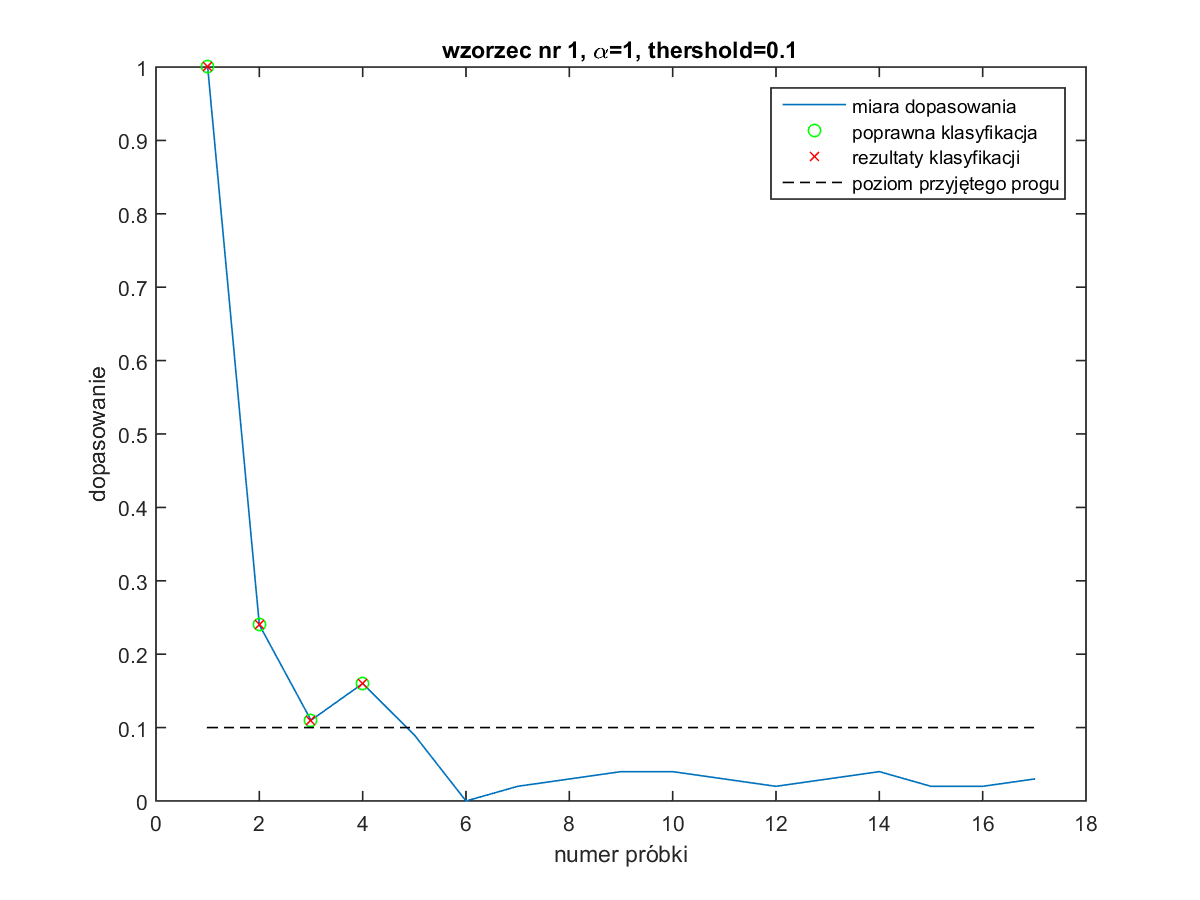
\includegraphics[width=0.8\linewidth]{second_rozpoznane/metric_1.png}
            \end{figure}
            \begin{figure}[H]
                \centering
                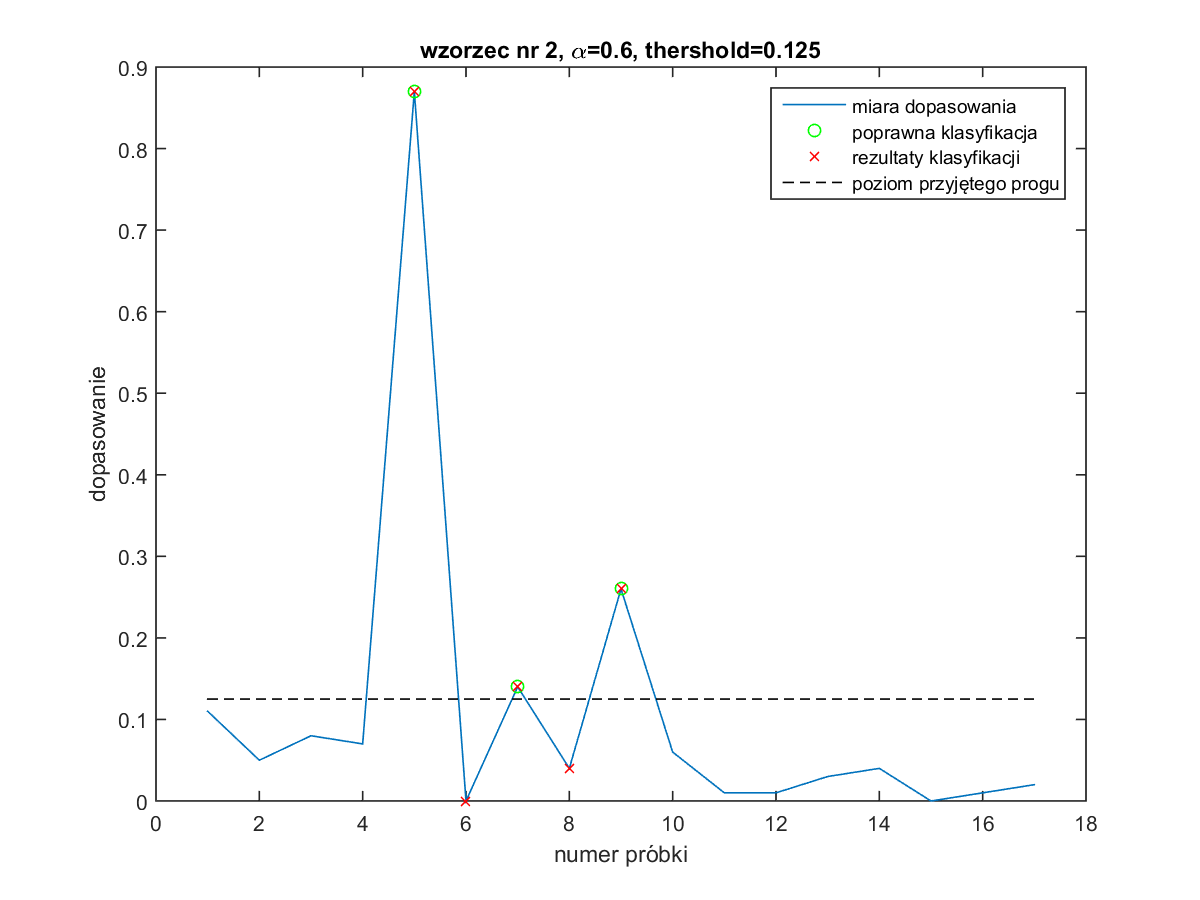
\includegraphics[width=0.8\linewidth]{second_rozpoznane/metric_2.png}
            \end{figure}
            \begin{figure}[H]
                \centering
                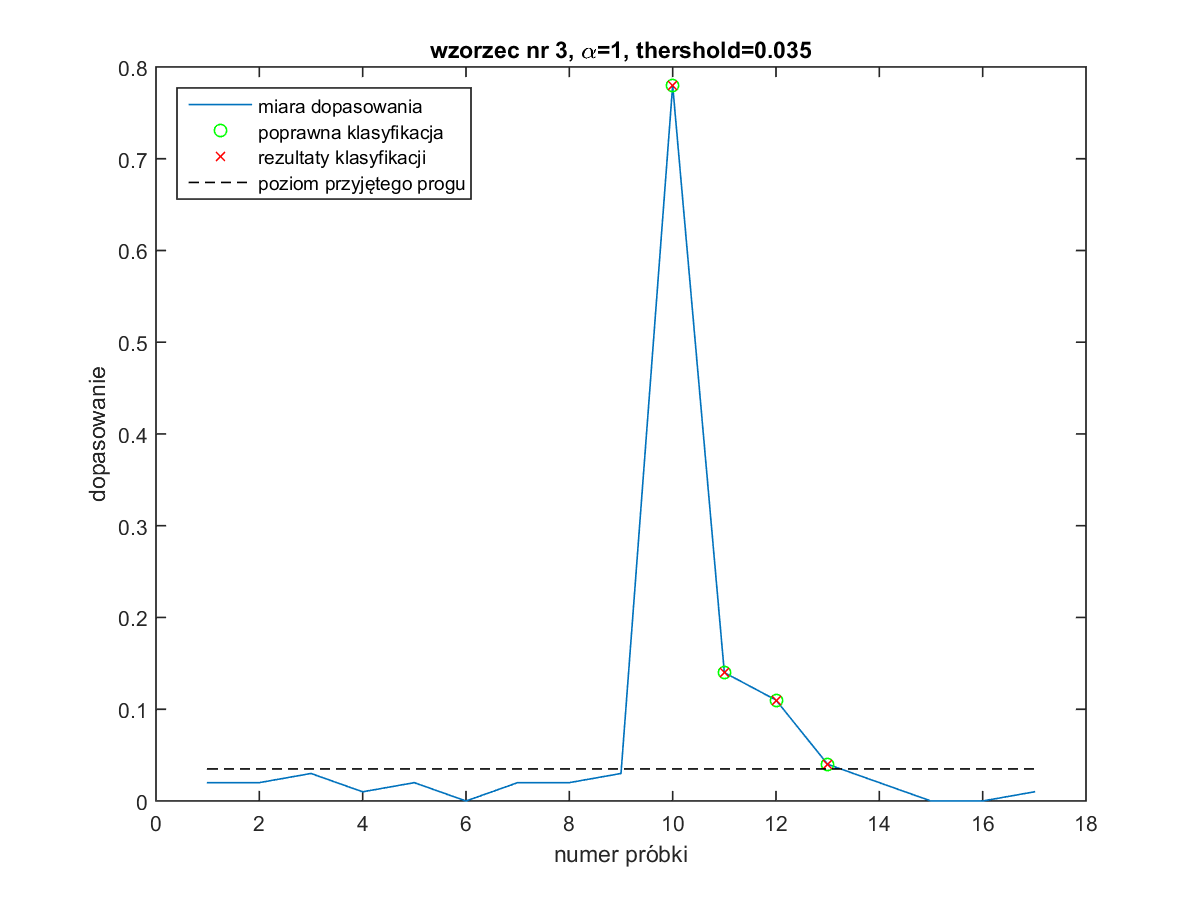
\includegraphics[width=0.8\linewidth]{second_rozpoznane/metric_3.png}
            \end{figure}
            \begin{figure}[H]
                \centering
                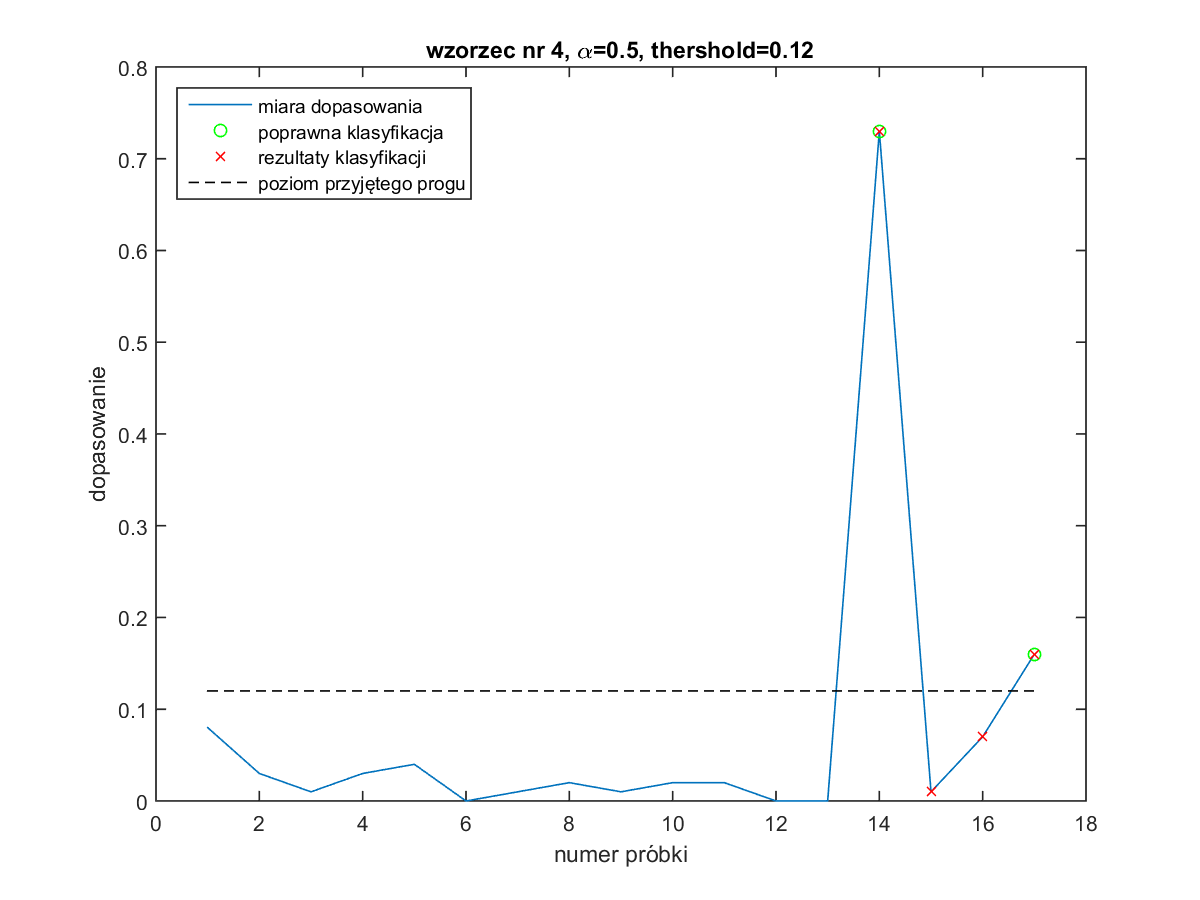
\includegraphics[width=0.8\linewidth]{second_rozpoznane/metric_4.png}
            \end{figure}
    \section{Rozpoznawanie na obrazie z wieloma elementami}            
        Rozpoznawanie zostało tu dokonane dokładnie tak jak w przypadku poprzedniego
        ćwiczenia. Po wynikach można zauważyć, że punkty są porozrzucane po kilku
        obiektach, a często mało z nich zostało wykrytych. Po zastosowaniu algorytmu
        RANSAC w dwóch przypadkach udało się poprawnie zlokalizować obiekt, a w 
        dwóch nie zadziałał (w jednym z powodu złego dobrania punktów, w drugim z 
        powodu zbyt małej liczby wykrytych punktów).
\begin{lstlisting}
[tform, inlierObjPoints, inlierScenePoints] = ...
    estimateGeometricTransform(matchedObjPoints,...
                               matchedScenePoints,...
                               'affine');

\end{lstlisting}
\begin{lstlisting}
figure;
showMatchedFeatures(objImage, sceneImage, inlierObjPoints, ...        
    inlierScenePoints, 'montage');

hold on;
[height, width] = size(objImage);
objPolygon = [
    1, 1;
    1, height;
    width, height;
    width, 1
];

[height, width] = size(sceneImage);
newObjPolygon = transformPointsForward(tform, objPolygon);
newObjPolygon = newObjPolygon';
newObjPolygon = [newObjPolygon, newObjPolygon(:, 1)];

plot(newObjPolygon(1,:) + width, newObjPolygon(2,:), 'g');
print(['third/second_' num2str(wzorzecNr)], '-dpng')
\end{lstlisting}
    \subsection{Wyniki}
        \begin{figure}[H]
            \centering
            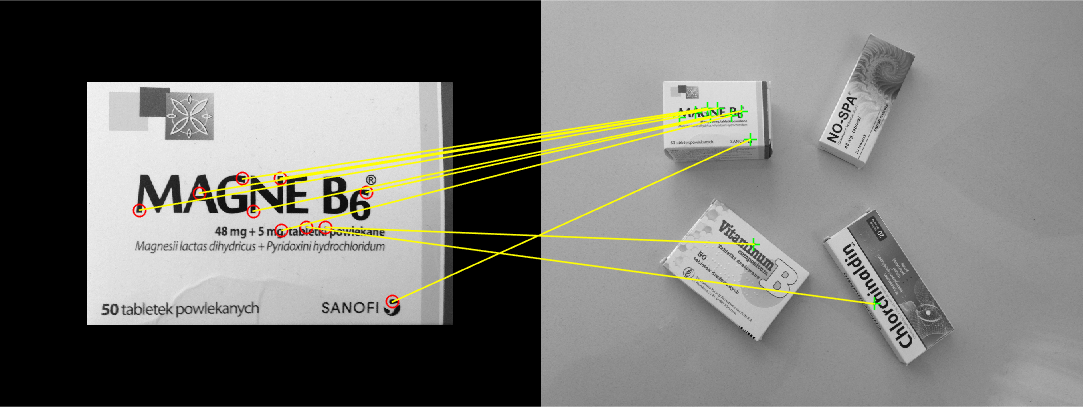
\includegraphics[width=0.8\linewidth]{third/first_1.png}
            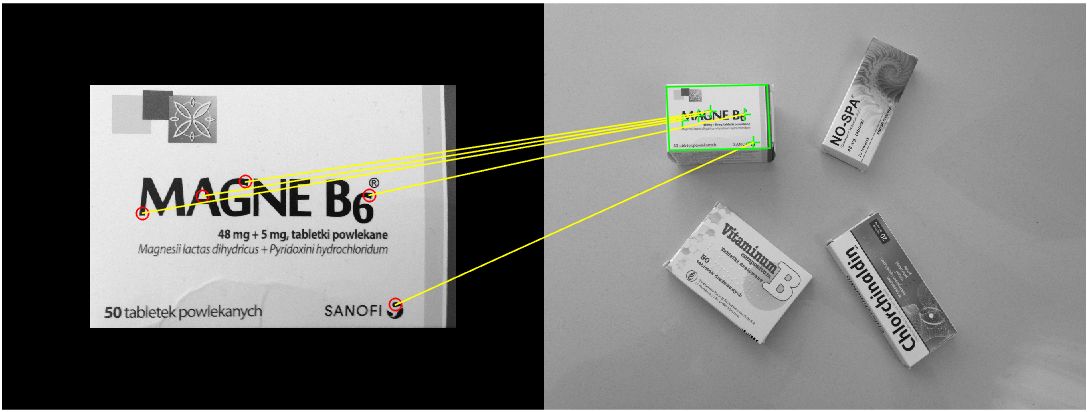
\includegraphics[width=0.8\linewidth]{third/second_1.png}
            \caption{MAGNE B6 -- poprawne wykrycie}
        \end{figure}
        \begin{figure}[H]
            \centering
            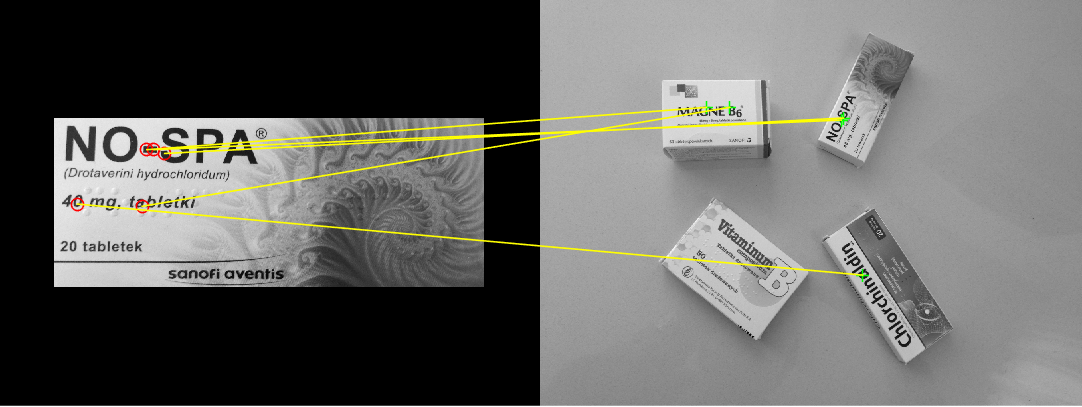
\includegraphics[width=0.8\linewidth]{third/first_2.png}
            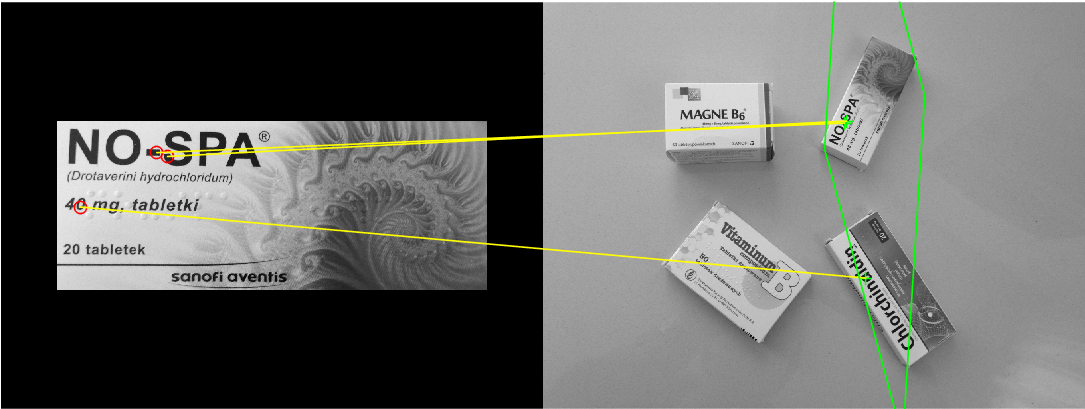
\includegraphics[width=0.8\linewidth]{third/second_2.png}
            \caption{NO-SPA -- błędne wykrycie}
        \end{figure}
        \begin{figure}[H]
            \centering
            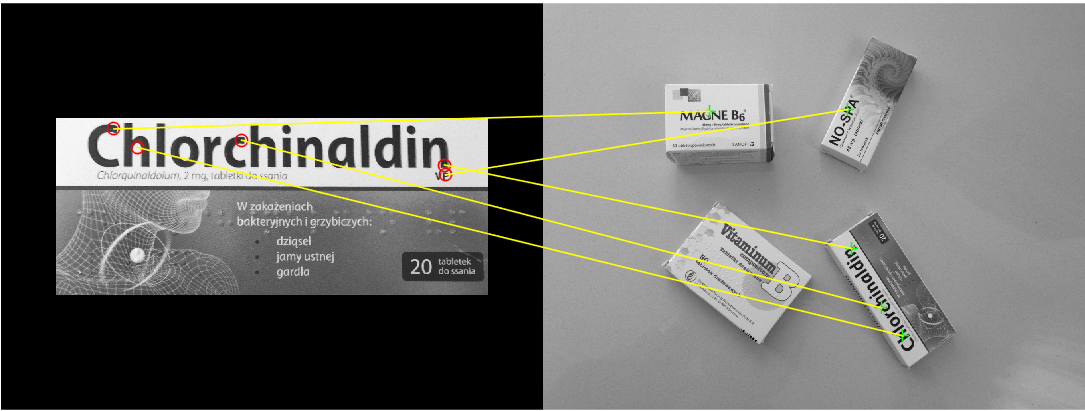
\includegraphics[width=0.8\linewidth]{third/first_3.png}
            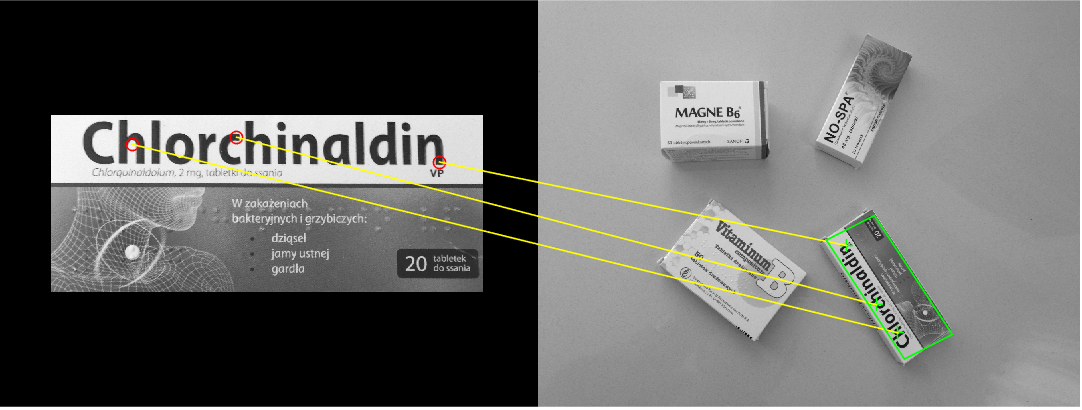
\includegraphics[width=0.8\linewidth]{third/second_3.png}
            \caption{Chlorochinaldin -- poprawne wykrycie mimo obrotu}
        \end{figure}
        \begin{figure}[H]
            \centering
            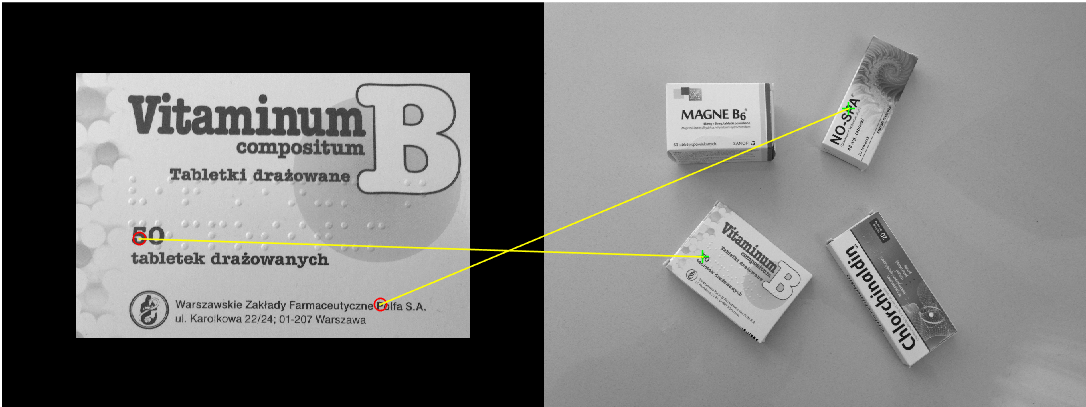
\includegraphics[width=0.8\linewidth]{third/first_4.png}
            \caption{Vitaminum B -- za mało punktów do przeprowadzenia RANSAC}
        \end{figure}
        
\end{document}
